\begin{frame}
\frametitle{Solutions of the Dirac equation for massless particles}
Define the right-handed and left-handed components of the Dirac spinor by:
\[
\psi_R = P_R \psi, \,\,\, \psi_L = P_L \psi
\]
with:
\[
P_R = \frac{1 + \gamma_5}{2}, \,\,\, P_L = \frac{1 - \gamma_5}{2}
\]
and
\[
\gamma^5 = i\gamma^0\gamma^1\gamma^2\gamma^3 
\]
which, in the Dirac representation equals:
\[
\gamma^5 = \mqty(\sigma_2 & 0 \\ 0 & -\sigma_2)
\]
Now, set the mass to zero in the Dirac equation, to get: 
\[
i \gamma^\mu \partial_\mu \psi = 0 \, \, \, (m=0)
\]
Then see that $\psi_R$~and $\psi_L$~also satisfy the massless Dirac equation
\end{frame}
\begin{frame}

\[
i \gamma^\mu \partial_\mu \psi_R = i \gamma^\mu P_R \partial_\mu \psi = 
P_L i \gamma^\mu \partial_\mu \psi = 0
\]
and the same result is found exchanging $P_R$~and $P_L$. This means that the right-handed and left-handed spinors satisfy \alert{independently} the Dirac equation. 
\[
i \gamma^\mu \partial_\mu \psi_R = 0 \, \, \, i \gamma^\mu \partial_\mu \psi_L = 0 \, \, \, (m=0)
\]
while if the mass is not zero they cannot be separated. 
\[
(i \gamma^\mu \partial_\mu - m) \psi_R =  i \gamma^\mu \partial_\mu \psi_R -m  \psi_R \ne 0
\]

\end{frame}

\begin{frame}
\frametitle{Weyl representation}
In the Weyl representation, the $\gamma$~matrices are chosen to be:
\[
\gamma^0 = \mqty(0 & I \\ I & 0), \,\,\,  \gamma^1 = \mqty(i \sigma_1 & 0 \\ 0 & i \sigma_1),
\gamma^2 = \mqty(0 & -\sigma_2 \\ \sigma_2 & 0), \,\,\,  
\gamma^3 = \mqty(i \sigma_3 & 0 \\ 0 & i \sigma_3)
\]
\[
\gamma^5 = \mqty(\sigma_2 & 0 \\ 0 & -\sigma_2) =  \mqty(I & 0 \\ 0 & -I)
\]
and 
\[
P_R =  \mqty(I & 0 \\ 0 & 0), \,\,\, P_L =  \mqty(0 & 0 \\ 0 & I)
\]
which means that $P_R$~ filters out the top two components and $P_R$~ filters out the bottom two components. Namely, in the Weyl representation the top half and the bottom half of the spinor transform independently under Lorentz transformations. 
\end{frame}
\begin{frame}
\frametitle{Helicity}
We define the helicity of a particle propagating with momentum $\va{p}$ as the spin projection in the
direction of $\va{p}$:
\[
h =  \frac{\va{\sigma}\cdot \va{p}}{\abs{p}} = (m \rightarrow 0) \gamma_5
\]
and 
\[
P_{R,L} = \frac{1 \pm \gamma_5}{2}
\]
\begin{itemize}
\item represents the helicity $\pm$~�projection operator for $e^-$.
\item represents the helicity $\mp$~�projection operator for $e^+$.
\end{itemize}

Since $\gamma_5$ and any (proper) Lorentz transformation  commute, once a state is an eigenstate of $\gamma_5$, one cannot change the eigenvalue of $\gamma_5$ by boosting it or rotating it.

\end{frame}

\begin{frame}
\frametitle{Masless particles have well defined helicity}
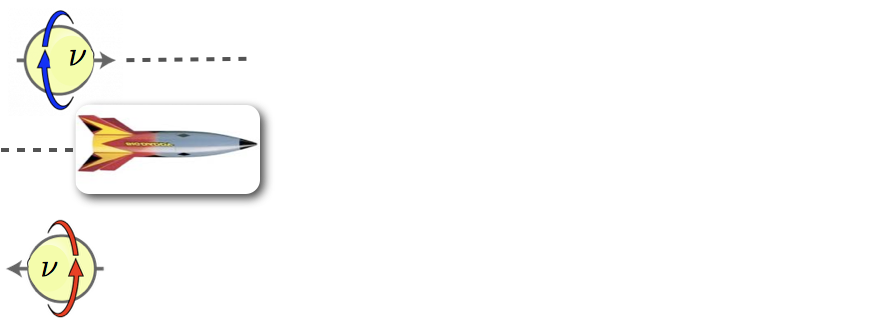
\includegraphics[scale=0.3]{neutrinoBoost2.png}

Namely, in the massless limit, one cannot change the value of helicity by boosting or rotating. This can be understood intuitively. The only way to reverse the spin component along the motion is for the observer to move faster than the particle and overtake it. Then, the direction of momentum viewed by the observer will flip while the spin will stay the same, and thus the helicity will change its sign. In the massless limit, the particle will be moving at the speed of light, and thus it is impossible to overtake it.

\end{frame}

\begin{frame}
\frametitle{Almost massless particles?}
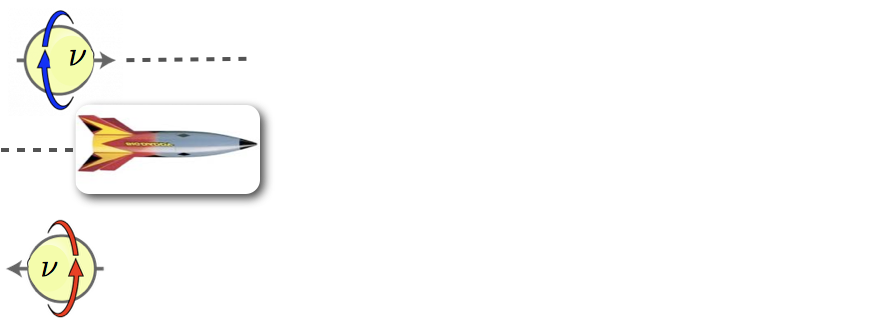
\includegraphics[scale=0.3]{neutrinoBoost2.png}

Experiments have established that the neutrino has a tiny mass. Thus, it moves ``almost'', but not quite at the speed of light, and one can reverse the argument before and jump into a boost that  ``overtakes'' the neutrino, thus see its helicity flip. Yet, the amount of ``wrong'' helicity that each one of the Weyl spinors has is very small, of the order $\frac{m}{E}$, where $m$~is the neutrino mass and $E$~its energy. 

\end{frame}

